\documentclass[aspectratio=169]{beamer}
\usetheme{Madrid}
\usecolortheme{beaver}
\usepackage[utf8]{inputenc}
\usepackage[T1]{fontenc}
\usepackage{tikz}
\usepackage{amssymb}
\usepackage{graphicx}
\setbeamertemplate{navigation symbols}{}
\setbeamercolor{title}{fg=white,bg=cyan!60!black}
\setbeamercolor{frametitle}{fg=white,bg=cyan!50!black}
\setbeamercolor{block title}{bg=cyan!15,fg=black}
\setbeamercolor{block body}{bg=cyan!5,fg=black}

\title{G10 — Design \& Capstone}
\subtitle{BOSS: Ship Your Own Game}
\author{ByteForge --- Grade 7 --- Game Maker}
\date{}

\begin{document}

\begin{frame}
    \titlepage
\end{frame}

\begin{frame}{FINAL BOSS — everything from the whole year}
    \Large
    A state machine, player input, a win condition, and at least one function you define — every major idea, combined into a game YOU designed.

    \begin{center}
    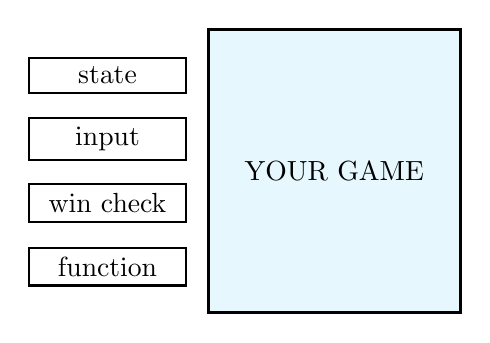
\begin{tikzpicture}[scale=0.9]

        \node[draw, thick, minimum width=2cm] at (0,0.9) {state};
        \node[draw, thick, minimum width=2cm] at (0,0) {input};
        \node[draw, thick, minimum width=2cm] at (0,-0.9) {win check};
        \node[draw, thick, minimum width=2cm] at (0,-1.8) {function};
        \node[draw, very thick, minimum width=3.2cm, minimum height=3.6cm, fill=cyan!10] at (3.2,-0.45) {YOUR GAME};
    \end{tikzpicture}
    \end{center}
\end{frame}

\begin{frame}{Playtest, then iterate}
    \Large
    Real developers ALWAYS playtest and adjust at least once — a first draft is rarely the final version.
\end{frame}

\begin{frame}{Your Turn}
    \Large
    Open the student map, find \textbf{G10 — Design \& Capstone}, and complete
    the \textbf{BOSS} challenge --- everything you just saw, they now do themselves.
\end{frame}

\end{document}
